\newpage
МРНТИ 61.71.29

\sectionwithauthors{Е.М. Сүлеймен}{КОМПОНЕНТНЫЙ СОСТАВ НЕФТИ МЕСТОРОЖДЕНИЯ УЗЕНЬ}

\begin{center}
{\bfseries \textsuperscript{1,2}Е.М. Сүлеймен}

\textsuperscript{1}Казахский университет технологии и бизнеса имени К.
Кулажанова, Астана, Казахстан,

\textsuperscript{2}ТОО «КМГ Инжиниринг», Астана, Казахстан,
\end{center}

Корреспондент-автор: Syerlan75@yandex.kz

Методом хромато-масс-спектрометрии исследован компонентный состав нефти
месторождения Узень. Для анализа использовали нефть, отобранную на
центральном пункте подготовки нефти, а также ее фракцию до 60 °С,
полученную при простой перегонке исходной нефти. Установлено, что кроме
традиционных основных компонентов нефти, в ней присутствует большое
содержание ценных ненасыщенных карбоновых кислот и их сложных эфиров. В
составе исследуемой нефти и ее фракции до 60 °С присутствует большое
количество метиловых эфиров Z,Z-9,12-октадекадиеновой (7.04 и 1.33
массовых \%) и Z-6-октадеценовой кислот (1.33 и 0.68 массовых \%)
соответственно. Данные вещества являются основой для производства
асидола и мылонафта. Также эти кислоты являются основой для биологически
активных добавок -- относятся к ω-кислотам. Составлена таблица ценных
компонентов нефти и представлены цена на некоторых из них.

{\bfseries Ключевые слова:} нефть, компонентный состав, месторождение
Узень, хромато-масс-спектрометрия, асидол, мылонафт, петроселиновая
кислота.

\sectionheading{ӨЗЕН КЕН ОРНЫНДАҒЫ МҰНАЙНЫҢ ӘДЕТТЕН ТЫС ҚҰРАМЫ ТУРАЛЫ}

\begin{center}
{\bfseries \textsuperscript{1,2}Е.М. Сүлеймен}

\textsuperscript{1}Қ. Құлажанов атындағы Қазақ технология және бизнес
университеті, Астана, Қазақстан,

\textsuperscript{2}«KMG Engineering» ЖШС, Астана, Қазақстан

e-mail: Syerlan75@yandex.kz
\end{center}

Өзен кен орнындағы мұнайдың компоненттік құрамы газды
хроматография-масс-спектрометрия әдісімен зерттелген. Талдау үшін біз
2020 жылдың 26 ақпанында орталық май тазарту станциясында сынама алынған
майды, сондай-ақ оның бастапқы майын қарапайым дистилляциялау
нәтижесінде алынған 60 ° C дейінгі фракциясын қолдандық. Мұнайдың
дәстүрлі негізгі компоненттерінен басқа құрамында құнды қанықпаған
карбон қышқылдары мен олардың эфирлерінің көп мөлшері бар екендігі
анықталды. Зерттелген мұнайдың құрамы мен оның 60 ° C дейінгі фракциясы
құрамында Z,Z-9,12-октадекадиен (массасылық \% 7,04 және 1,33\%) және
Z-6-октадецен қышқылдарының сәйкесінше (массалық \% 1,33 және 0,68)
метил эфирлерінің мөлшері бар. Бұл заттар асидол мен мылонафт шығарудың
негізі болып табылады. Сондай-ақ, бұл қышқылдар тағамдық қоспалардың
негізі болып табылады - олар ω-қышқылдарға жатады. Мұнайдың бағалы
компоненттерінің кестесі жасалды және олардың кейбіреулеріне бағалар
ұсынылды.

{\bfseries Түйін сөздер}: мұнай, құрамы, Өзен кен орны, газ
хроматография-масс-спектрометриясы, асидол, милонафт, петроселин
қышқылы.

\sectionheading{ABOUT THE UNUSUAL OIL COMPOSITION OF THE UZEN FIELD}

\begin{center}
{\bfseries \textsuperscript{1,2}Ye.M. Suleimen}

\textsuperscript{1}Kazakh University of Technology and Business named
after K. Kulazhanov, Astana, Kazakhstan,

\textsuperscript{2}KMG Engineering LLP, Astana, Kazakhstan

e-mail: Syerlan75@yandex.kz
\end{center}

The compositional composition of oil from the Uzen field has been
studied by gas chromatography-mass spectrometry. For the analysis, we
used the oil sampled at the central oil treatment station on February
26, 2020, as well as its fraction up to 60 °C, obtained by simple
distillation of the original oil. It was found that in addition to the
traditional main components of oil, it contains a high content of
valuable unsaturated carboxylic acids and their esters. The composition
of the studied oil and its fraction up to 60 °C contains a large amount
of methyl esters of Z, Z-9,12-octadecadienoic (7.04 and 1.33 mass\%) and
Z-6-octadecenoic acids (1.33 and 0.68 mass\%), respectively. These
substances are the basis for the production of acidol and mylonaft.
Also, these acids are the basis for dietary supplements - they belong to
ω-acids. A table of valuable oil components has been compiled and the
price of some of them is presented.

{\bfseries Key words:} oil, composition, Uzen field, gas
chromatography-mass spectrometry, asidol, mylonaft, petroselinic acid.

\begin{multicols}{2}
{\bfseries Введение.} Сжигать нефть -- одно и тоже, что сжигать
ассигнации», говорил известный ученый Д.И. Менделеев. Одними из ценных
веществ, находящихся в составе нефти, являются нафтеновые кислоты. Из
данных кислот производят в промышленном масштабе, пластификаторы
бетонов, ценные лекарственные вещества, смазочные материалы, сырье для
моющих материалов, такие как асидол и мылонафт, и многое другое {[}1{]}.
Следует отметить, до недавнего времени считалось, что наиболее богатые
нафтеновыми кислотами, являются бакинские нефти, в которых содержание
достигает 1-2\% {[}2{]}.

АО «Озенмунайгаз» - 100-процентная дочерняя компания АО НК
«КазМунайГаз». В 2020 году предприятие занимало 6\% в структуре~добычи
нефти и газоконденсата в Казахстане. Предприятие занимается добычей
нефти и газоконденсата на месторождениях Узень и Карамандыбас в
Мангистауской области.

Месторождение Узень -- одно из крупнейших месторождений с уникальными
начальными геологическими запасами не только в Республике Казахстан, но
и во всем мире. Это многопластовое месторождение со сложным строением,
залежи нефти и газа, которых сосредоточены в терригенном разрезе
юрско-меловых отложений.

На месторождении Узень в Мангистауской области путем доразведки в 2022
году обнаружены новые залежи нефти. В результате прирост извлекаемых
запасов нефти составил 39,9 млн тонн {[}3{]}.

В связи с этим проявляется и интерес к компонентному составу нефти
данного месторождения.

В литературе мы не обнаружили данные по компонентному составу нефти
месторождения Узень.

С другой стороны ранее использованные методы по определению
компонентного состава, такие как перегонка и газовая хроматография, были
трудоемки и менее достоверны по сравнению с таким новым методом, таким
как хромато-масс-спектрометрия.

Целью настоящей работы является исследование компонентного состава нефти
месторождения Узень и применимость ее в различных сферах применения.

Для исследования компонентного состава использовали метод
хромато-масс-спектрометрии.

{\bfseries Материалы и методы.} Для анализа использовали общую нефть, а
также полученную разгонкой при атмосферном давлении на бане с
вазелиновым маслом. В этом случае отбирали фракцию до 60 \emph{°}С.
Объем нефти, взятой для перегонки 100 мл и получили фракцию нефти до 60
\emph{°}С массой 7 мл. Таким образом выход фракции нефти, полученной
перегонкой до 60 \emph{°}С, составил 7\% (по объему) (рисунок 1). Нефть
и фракцию нефти до 60~\emph{°}С, предназначенные для анализа, растворяли
в гексане.

Определение компонентного состава нефти и фракции нефти, полученной
перегонкой до 60 \textsuperscript{о}С, проводили на газовом хроматографе
Clarus-SQ 8 с масс-спектрометрическим детектором. Хроматографические
условия: колонка капиллярная RestekRxi®-1 ms 0,25 мм х 30 м х 0,25 мкм;
объем пробы: 1,0 мкл; газ-носитель: Не; скорость газа-носителя: 1
мл/мин; деление потока 1:25; t колонки: 45 \textsuperscript{о}С (2 мин),
подъем 1,5 ~С/мин до 200 \textsuperscript{о}С, далее 15
\textsuperscript{о}С/мин до 280 \textsuperscript{о}С, изотермический
режим при 280\textsuperscript{о}С в течение 10 мин; t испарителя -- 280
\textsuperscript{о}С, масс-спектрометрический детектор: t -- 240
\textsuperscript{о}С, EI+ = 70 eB; время сканирования с 4 по 120 мин;
режим сканирования ионов: 39--500 ~m/z. Процентное содержание
компонентов вычисляли автоматически, исходя из площадей пиков общей
хроматограммы ионов. Компоненты идентифицировали по масс-спектрам и
временам удерживания, с использованием библиотеки NIST. Время
удерживания компонентов пересчитывали относительно предельных
углеводородов (рисунок 2).
\end{multicols}

% \begin{longtable}[]{@{}
%   >{\raggedright\arraybackslash}p{(\columnwidth - 2\tabcolsep) * \real{0.3819}}
%   >{\raggedright\arraybackslash}p{(\columnwidth - 2\tabcolsep) * \real{0.6181}}@{}}
% \toprule\noalign{}
% \begin{minipage}[b]{\linewidth}\raggedright
% \begin{figure}[H]
% 	\centering
% 	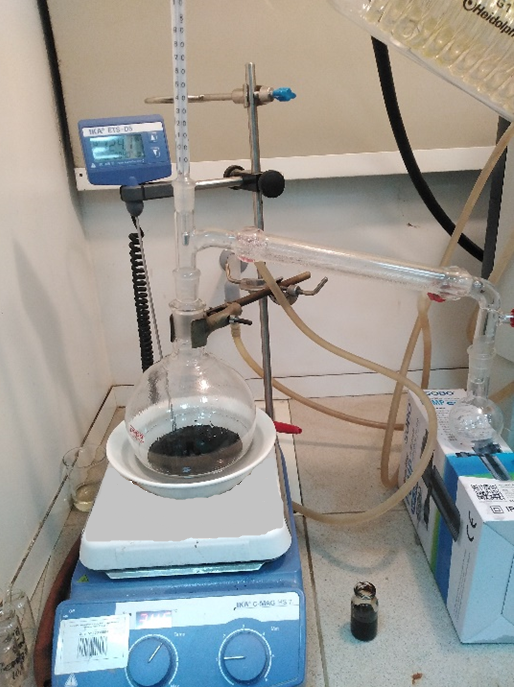
\includegraphics[width=0.8\textwidth]{assets/368}
% 	\caption*{}
% \end{figure}
% \end{minipage} & \begin{minipage}[b]{\linewidth}\raggedright
% \begin{figure}[H]
% 	\centering
% 	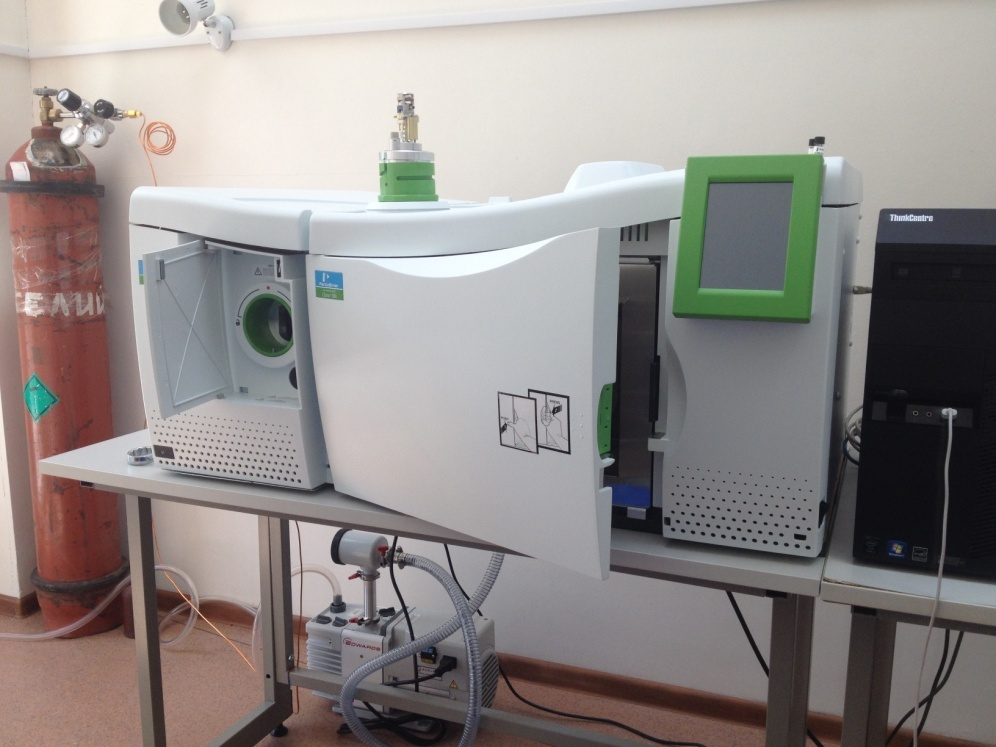
\includegraphics[width=0.8\textwidth]{assets/369}
% 	\caption*{}
% \end{figure}
% \end{minipage} \\
% \midrule\noalign{}
% \endhead
% \bottomrule\noalign{}
% \endlastfoot
% {\bfseries Рис.1 -Перегонка нефти под}
% 
% {\bfseries атмосферным давлением} & {\bfseries Рис.2 - Анализ нефти и фракции
% нефти до 60 \emph{°}С}
% 
% {\bfseries методом хромато-масс-спектрометрии} \\
% \end{longtable}

{\bfseries Результаты и обсуждение.} Как видно из рисунков 3-4 и таблицы 1,
состав нефти представлен следующими основными компонентами (представлены
основные 5 компонентов или выше 3\%):

\begin{enumerate}
\def\labelenumi{\arabic{enumi}.}
\item
  В нефти: нонан 15,78\%, (\emph{Z,Z})-9,12-октадекадиеновой кислоты
  метиловый эфир -7,04\%, октадекан - 3,96\%, (\emph{Z})-6-октадекановой
  кислоты метиловый эфир - 2,82\% и пентадекан - 2,70\%. В нефти
  нормальные углеводороды составляют 70\% от общего количества
  компонентов, циклические -- 12\%, далее кислоты -- до 11\% и
  незначительное содержание ароматических углеводородов -- 1\%. 3\%
  составляют неидентифицированные компоненты (часть из них, возможно,
  стерины).
\item
  Во фракции нефти, полученной перегонкой до 60 °С: октан - 18,67\%,
  толуол- 12,74\%, 1,3-диметилциклогексан - 7,53\%, нонан - 6,50\%,
  3-метилгептан - 5,72\%, 1,3-диметилбензол - 4,19\% и
  1,4-диметилциклогексан - 3,03\%. В этой фракции нормальные
  углеводороды составляют 42\% от общего количества компонентов,
  циклические -- 38\%, далее ароматические углеводороды -- до 17\% и
  незначительное содержание кислот (2\%) и ненасыщенных соединений
  (0,5\%).
\end{enumerate}

Как видно из таблицы, нами же методом хромато-масс-спектрометрии изучен
состав нефти Узеньского месторождения и установлено, что в составе
содержатся метилированные производные нафтеновых кислот до 11\%, причем
3\% - омега-12 карбоновая кислота. Именно весьма ценным и перспективным
в исследуемой нефти является присутствие омега-12 карбоновой кислоты -
петроселиновой кислоты, которые обнаружены нами в необычном компонентном
составе нефти месторождения Узень.

В литературе нами не обнаружены данные по детальному компонентному
составу нефти Узеньского месторождения методом
хромато-масс-спектрометрии. В публикациях представлен лишь общее
содержание групповых фракций: углеводороды, ароматические соединения и
т.д. {[}4-5{]}.

\begin{figure}[H]
	\centering
	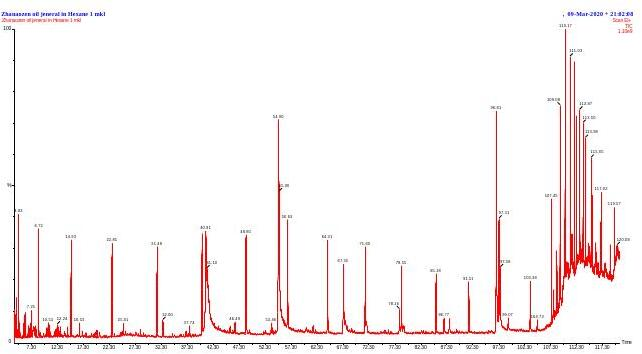
\includegraphics[width=0.8\textwidth]{assets/370}
	\caption*{}
\end{figure}10.58805/kazutb.v.3.24-569

{\bfseries Рис. 3 - Хроматограмма компонентного состава нефти без разгонки}

\begin{figure}[H]
	\centering
	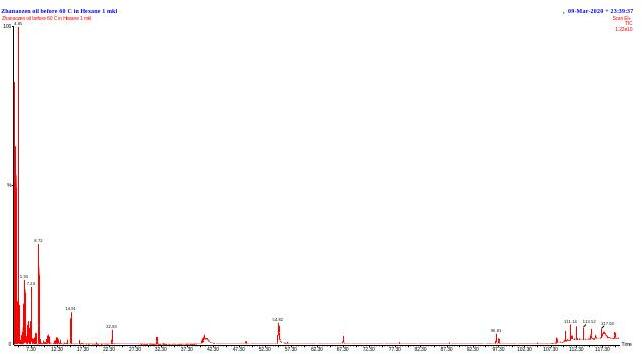
\includegraphics[width=0.8\textwidth]{assets/371}
	\caption*{}
\end{figure}

{\bfseries Рис. 4- Хроматограмма компонентного состава нефти фракции до 60
\textsuperscript{о}С}

Омега-12 карбоновые кислоты (рисунок 5) найдены в масле грецкого ореха,
в кукурузном, подсолнечном, соевом, хлопковом маслах, семенах тыквы.
Следует отметить, что омега-12 карбоновая кислота (петроселиновая
кислота) -- в основном содержится в маслах кориандровых растений
{[}6{]}. Достаточно хорошо изучена ферментативная активность ряда омега
кислот {[}7{]}. Известно, что омега-12 кислоты снижают уровень жиров в
организме {[}8{]}.

\begin{figure}[H]
	\centering
	
\includegraphics[width=0.8\textwidth]{assets/372}
	\caption*{}
\end{figure}

{\bfseries Рис. 5- Петроселиновая кислота}

{\bfseries Таблица 1 - Компонентный состав нефти месторождения Узень}

\begin{longtable}[]{@{}
  >{\raggedright\arraybackslash}p{(\columnwidth - 12\tabcolsep) * \real{0.1042}}
  >{\raggedright\arraybackslash}p{(\columnwidth - 12\tabcolsep) * \real{0.1111}}
  >{\raggedright\arraybackslash}p{(\columnwidth - 12\tabcolsep) * \real{0.0826}}
  >{\raggedright\arraybackslash}p{(\columnwidth - 12\tabcolsep) * \real{0.4694}}
  >{\raggedright\arraybackslash}p{(\columnwidth - 12\tabcolsep) * \real{0.0872}}
  >{\raggedright\arraybackslash}p{(\columnwidth - 12\tabcolsep) * \real{0.0728}}
  >{\raggedright\arraybackslash}p{(\columnwidth - 12\tabcolsep) * \real{0.0726}}@{}}
\toprule\noalign{}
\endhead
\bottomrule\noalign{}
\endlastfoot
\multirow{2}{=}{RT} & \multirow{2}{=}{Rлит.} & \multirow{2}{=}{Rвыч.} &
\multirow{2}{=}{Компонент} & \multirow{2}{=}{Cоотве-тствие} &
\multicolumn{2}{>{\raggedright\arraybackslash}p{(\columnwidth - 12\tabcolsep) * \real{0.1454} + 2\tabcolsep}@{}} \\
& & & & & A & B \\
{\bfseries 4.029} & {\bfseries 763±8} & {\bfseries 776} & {\bfseries Толуол*,**} &
{\bfseries 905} & {\bfseries 0,06} & {\bfseries 11,18} \\
{\bfseries 4.143} & {\bfseries 773±1} & {\bfseries 779} &
{\bfseries 3-Метилгептан***} & {\bfseries 904} & {\bfseries 0,19} &
{\bfseries 5,02} \\
4.22 & 776±2 & 781 & \emph{цис}-1,1,3,4-Тераметилциклопентан**** & 864 &
& 0,46 \\
{\bfseries 4.341} & {\bfseries 796±12} & {\bfseries 784} &
{\bfseries 1,3-Диметилциклогексан} & {\bfseries 913} & {\bfseries 0,31} &
{\bfseries 6,61} \\
{\bfseries 4.411} & {\bfseries 805±4} & {\bfseries 786} &
{\bfseries 1,4-Диметилциклогексан} & {\bfseries 914} & {\bfseries 0,12} &
{\bfseries 2,66} \\
4.554 & 791±4 & 790 & 1,1-Диметилциклогексан & 714 & 0,06 & 1,42 \\
4.642 & 793±3 & 792 & \emph{транс}-1-Этил-2-метилциклопентан & 847 &
0,06 & 1,35 \\
4.741 & 797±4 & 794 & 1-Этил-1-метилциклопентан & 911 & & 0,10 \\
{\bfseries 4.825} & {\bfseries 800} & {\bfseries 797} & {\bfseries Октан} &
{\bfseries 953} & {\bfseries 1,14} & {\bfseries 16,39} \\
5.042 & 807±3 & 802 & \emph{транс}-1,3-Диметилциклогексан & 918 & &
1,36 \\
5.045 & 810±5 & 802 & 1,4-Диметилциклогексан & 854 & 0,09 & \\
5.163 & 818±4 & 805 & \emph{цис}-1,1,3,4-Тераметилциклопентан & 844 & &
0,13 \\
5.221 & 817±5 & 807 & 1-Метиоэтилциклопентан & 786 & & 0,16 \\
5.353 & 824±2 & 810 & 3-Этил-2,2-диэтилпентан & 858 & & 0,29 \\
5.456 & 821±1 & 813 & 2,4-Диэтилгептан & 951 & & 0,32 \\
5.533 & 825±4 & 815 & \emph{цис}-1-Этил-3-метилциклопентан & 842 & &
0,13 \\
5.651 & & 818 & \emph{Неизвестное соединение 1*****} & & & 0,17 \\
5.706 & 827±1 & 819 & 2,6-Диметилгептан & 884 & 0,13 & 1,51 \\
5.794 & 833±5 & 822 & \emph{цис}-1,2-Диметилциклогексан & 917 & &
0,25 \\
5.838 & 834±3 & 823 & Пропилциклогексан & 732 & & 0,39 \\
{\bfseries 5.926} & {\bfseries 836±5} & {\bfseries 825} &
{\bfseries Этилциклогексан} & {\bfseries 850} & {\bfseries 0,25} &
{\bfseries 2,53} \\
{\bfseries 6.073} & {\bfseries 844±4} & {\bfseries 829} &
{\bfseries 1,1,3-Триметилциклогексан} & {\bfseries 900} & {\bfseries 0,25} &
{\bfseries 2,21} \\
6.186 & 842±4 & 832 & 1,1,4-Триметилциклогексан & 857 & & 0,25 \\
6.252 & 849±4 & 833 & 1,2,4-Триметилциклогексан & 729 & & 0,20 \\
6.454 & 853±0 & 839 & 6-Метил-1-октен****** & 840 & & 0,30 \\
6.649 & 853±3 & 844 & 1,3,5-Триметилциклогексан & 868 & 0,12 & 0,79 \\
6.711 & 855±1 & 845 & 2,3-Диметигептан & 874 & 0,13 & 0,86 \\
6.872 & 855±10 & 849 & Этилбензол & 736 & 0,06 & 0,60 \\
7.023 & 863±1 & 853 & 4-Метилоктан & 834 & 0,09 & 0,58 \\
7.096 & 865±1 & 855 & 2-Метилоктан & 872 & 0,13 & 0,91 \\
{\bfseries 7.254} & {\bfseries 866±7} & {\bfseries 859} &
{\bfseries 1,3-Диметилбензол} & {\bfseries 915} & {\bfseries 0,41} &
{\bfseries 3,68} \\
7.368 & 871±1 & 862 & 3-Метилоктан & 850 & 0,24 & 1,30 \\
7.925 & 877±9 & 877 & 1,2,3-Триметил-(1α,2β,3α)-циклогексан & 740 & 0,96
& 0,08 \\
7.584 & 877±9 & 868 & 1,2,3-Триметил-(1α,2β,3α)-циклогексан & 901 & &
0,38 \\
7.775 & 877±3 & 873 & 1,2,4-Триметил-(1α,2β,4β)-циклогексан & 871 & &
0,05 \\
7.914 & 887±5 & 876 & 1,1,2-Триметилциклогексан & 798 & & 0,33 \\
7.966 & 889±3 & 878 & 1-Нонен & 853 & & 0,13 \\
8.12 & 894±4 & 882 & \emph{цис}-1-Этил-3-метилциклогексан & 849 & 1,42 &
0,56 \\
8.274 & 896±4 & 886 & \emph{транс}-1-Этил-4-метилциклогексан & 638 &
1,92 & 0,97 \\
{\bfseries 8.718} & {\bfseries 900} & {\bfseries 897} & {\bfseries Нонан} &
{\bfseries 912} & {\bfseries 15,78} & {\bfseries 5,70} \\
8.901 & 908±25 & 901 & 1,2,3-Триметил-(1α,2α,3β)-циклогексан & 776 & &
0,07 \\
9.037 & 919±N/A & 903 & 1-Этил-2-метилциклогексан & 915 & & 0,32 \\
9.048 & 910±4 & 903 & \emph{цис}-1-Этил-4-метилциклогексан & 724 & 1,20
& 0,13 \\
9.459 & 919±0 & 910 & 2,3,6-Триметилгептан & 817 & & 0,05 \\
9.558 & 919±1 & 911 & 4,4-Диметилоктан & 744 & & 0,09 \\
9.646 & 930±N/A & 913 & Октагидро-1-метилпентален* & 712 & 1,17 &
0,25 \\
9.829 & 921±9 & 915 & Кумол & 789 & & 0,07 \\
9.961 & 922±1 & 917 & 3,5-Диметилоктан & 818 & & 0,15 \\
10.288 & 931±5 & 922 & Пропилциклогексан & 829 & 1,68 & 0,47 \\
{\bfseries 10.534} & {\bfseries 933±2} & {\bfseries 926} &
{\bfseries 2,6-Диметилоктан} & {\bfseries 893} & {\bfseries 2,66} &
{\bfseries 0,64} \\
\multirow{2}{=}{RT} & \multirow{2}{=}{Rлит.} & \multirow{2}{=}{Rвыч.} &
\multirow{2}{=}{Компонент} & \multirow{2}{=}{Соотве-тствие} &
\multicolumn{2}{>{\raggedright\arraybackslash}p{(\columnwidth - 12\tabcolsep) * \real{0.1454} + 2\tabcolsep}@{}} \\
& & & & & A & B \\
{\bfseries 10.838} & {\bfseries 941±1} & {\bfseries 931} &
{\bfseries 3-Этил-2-метилгептан} & {\bfseries 873} & {\bfseries 2,35} &
{\bfseries 0,54} \\
10.934 & 958±1 & 932 & 1,1,2,3-Тетраметилциклогексан & 824 & & 0,09 \\
11.176 & 987±3 & 936 & 1-Децин & 777 & & 0,08 \\
11.554 & 953±10 & 942 & Пропилбензол & 774 & & 0,08 \\
11.77 & 952±1 & 945 & 4-Этилоктан & 718 & 1,08 & 0,19 \\
11.854 & 958±1 & 946 & 1,1,2,3-Тетраметилциклогексан & 868 & 1,39 &
0,20 \\
12.067 & 957±8 & 950 & 1-Этил-3-метилбензол & 752 & 0,15 & 0,33 \\
12.24 & 953±1 & 952 & 2,3-Диметилоктан & 717 & 0,22 & 0,45 \\
12.474 & 964±1 & 956 & 2-Метилнонан & 821 & 0,16 & 0,27 \\
12.595 & 972±9 & 958 & Мезитилен & 808 & 0,09 & 0,17 \\
12.878 & 965±1 & 962 & 3-Этилоктан & 729 & 0,22 & 0,33 \\
13.116 & 957±8 & 966 & 1-Этил-3-метилбензол & 703 & & 0,15 \\
13.619 & 983±0 & 973 & 1-Метил-2-пропилциклогексан & 859 & 0,12 &
0,19 \\
14.213 & 990±6 & 983 & 1,2,3-Триметилбензол & 895 & 0,22 & 0,19 \\
14.463 & 990±N/A & 986 & \emph{м}-Ментан & 738 & & 12,69 \\
{\bfseries 14.929} & {\bfseries 1000} & {\bfseries 994} & {\bfseries Декан} &
{\bfseries 899} & {\bfseries 1,71} & {\bfseries 2,32} \\
15.31 & 1042 iu & 999 & 9-Метилбицикло{[}3.3.1{]}нонан & 633 & & 0,05 \\
16.051 & 1013±7 & 1009 & 1,2,3-Триметилбензол & 868 & & 0,08 \\
16.528 & 1018±2 & 1015 & 2,6-Диметилнонан & 871 & 0,33 & 0,32 \\
17.097 & 1030±2 & 1023 & Бутилциклогексан & 722 & 0,15 & 0,12 \\
17.765 & 1066 iu & 1031 & 5-Метил-2-(1-метилэтил)-1-гексанол & 760 &
0,12 & 0,10 \\
18.436 & 1037±6 & 1040 & 1-Метил-2-пропилбензол & 793 & & 0,04 \\
18.792 & 1056±7 & 1044 & \emph{транс}-Декагидронафталин & 724 & 0,13 &
0,12 \\
19.225 & 1057±1 & 1050 & 5-Метилдекан & 801 & 0,07 & 0,07 \\
19.529 & 1060±1 & 1054 & 4-Метилдекан & 722 & 0,13 & 0,10 \\
19.878 & 1064±2 & 1059 & 2-Метилдекан & 882 & 0,18 & 0,15 \\
20.362 & 1071±1 & 1065 & 3-Метилдекан & 757 & 0,21 & 0,13 \\
21.25 & 1040 iu & 1077 & 1-Метил-3-пропилциклогексан & 757 & 0,07 & \\
22.846 & 1100 & 1098 & Ундекан & 889 & 1,97 & 1,24 \\
24.548 & 1129±14 & 1117 & Декагидро-2-метилнафталин & 824 & 0,12 &
0,04 \\
25.032 & 1125±1 & 1122 & 3,7-Диметилдекан & 743 & & 0,04 \\
25.432 & 1135±3 & 1126 & Пентилциклогексан & 767 & & 0,05 \\
27.535 & 1156±1 & 1149 & 5-Метилундекан & 704 & 0,10 & \\
28.331 & 1164±1 & 1158 & 2-Метилундекан & 726 & 0,18 & 0,07 \\
28.852 & 1170±1 & 1163 & 3-Метилундекан & 803 & 0,09 & 0,04 \\
{\bfseries 31.482} & {\bfseries 1200} & {\bfseries 1192} & {\bfseries Додекан} &
{\bfseries 908} & {\bfseries 2,14} & {\bfseries 0,74} \\
32.597 & 1210±4 & 1205 & 2,6-Диметилундекан & 886 & 0,43 & 0,13 \\
34.446 & 1238±2 & 1227 & Гексилциклогексан & 764 & 0,10 & \\
37.04 & 1264±2 & 1259 & 2-Метилдодекан & 829 & 0,13 & \\
37.554 & 1271±1 & 1265 & 3-Метилдодекан & 728 & 0,10 & \\
37.745 & 1275±N/A & 1268 & 2,6,11-Триметилдодекан & 788 & 0,30 & 0,07 \\
{\bfseries 40.181} & {\bfseries 1300} & {\bfseries 1297} & {\bfseries Тридекан} &
{\bfseries 872} & {\bfseries 2,28} & {\bfseries 0,42} \\
43.354 & 1346±2 & 1335 & Гептилциклогексан & 739 & 0,41 & \\
45.552 & 1364±1 & 1361 & 2-Метилтридекан & 769 & 0,41 & \\
46.073 & 1371±1 & 1367 & 3-Метилтридекан & 716 & 0,06 & \\
46.494 & 1366±2 & 1372 & 2,7,10-Триметилдодекан & 855 & 0,33 & \\
{\bfseries 48.597} & {\bfseries 1400} & {\bfseries 1397} & {\bfseries Тетрадекан} &
{\bfseries 884} & {\bfseries 2,53} & {\bfseries 0,30} \\
49.29 & 1427±0 & 1405 &
\emph{транс}-Октагидро-2,2,4,4,7,7-гексаметил-1Н-инден & 728 & 0,13 & \\
52.291 & 1472±2 & 1439 & Декагидро-1,1,4a,5,6-пентаметилнафталин & 749 &
0,10 & \\
53.465 & 1449±1 & 1452 & 2,6,10-Триметилтридекан & 843 & 0,34 & \\
\multirow{2}{=}{RT} & \multirow{2}{=}{Rлит.} & \multirow{2}{=}{Rвыч.} &
\multirow{2}{=}{Компонент} & \multirow{2}{=}{Соотве-тствие} &
\multicolumn{2}{>{\raggedright\arraybackslash}p{(\columnwidth - 12\tabcolsep) * \real{0.1454} + 2\tabcolsep}@{}} \\
& & & & & A & B \\
54.232 & 1470±1 & 1461 & 3-Метилтетрадекан & 587 & 0,06 & \\
{\bfseries 56.635} & {\bfseries 1500} & {\bfseries 1488} & {\bfseries Пентадекан} &
{\bfseries 888} & {\bfseries 2,70} & {\bfseries 0,19} \\
61.536 & 1563±1 & 1556 & 2-Метилпентадекан & 766 & 0,25 & \\
{\bfseries 64.306} & {\bfseries 1600} & {\bfseries 1597} & {\bfseries Гексадекан} &
{\bfseries 882} & {\bfseries 2,44} & {\bfseries 0,08} \\
68.954 & 1664±1 & 1665 & 2-Метилгексадекан & 743 & 0,13 & \\
{\bfseries 71.596} & {\bfseries 1700} & {\bfseries 1704} & {\bfseries Гептадекан} &
{\bfseries 890} & {\bfseries 2,23} & \\
71.794 & 1687±5 & 1707 & 2,6,10,14-Тетраметилпентадекан & 783 & 0,34
& \\
71.889 & 1727±1 & 1708 & 2,6,10-Триметилгексадекан & 749 & 0,33 & \\
76.024 & 1765±1 & 1769 & 2-Метилгептадекан & 769 & 0,12 & \\
{\bfseries 78.548} & {\bfseries 1800} & {\bfseries 1806} & {\bfseries Октадекан} &
{\bfseries 875} & {\bfseries 3,96} & \\
78.896 & 1863±3 & 1811 & 2-Метилоктадекан & 691 & 0,43 & \\
79.003 & 1889±4 & 1812 & 2,6,10,15-Тетраметилгептадекан & 705 & 0,50
& \\
85.181 & 1900 & 1903 & Нонадекан & 922 & 1,66 & \\
86.766 & 1926±2 & 1926 & Метиловый эфир пальмитиновой кислоты****** &
867 & 0,53 & 0,05 \\
91.509 & 2000 & 1995 & Эйкозан & 858 & 1,45 & 0,00 \\
{\bfseries 96.811} & {\bfseries 2092±4} & {\bfseries 2084} & {\bfseries Метиловый
эфир (Z, Z) 9,12-октадекадиеновой кислота} & {\bfseries 909} &
{\bfseries 7,04} & {\bfseries 1,33} \\
{\bfseries 97.31} & {\bfseries 2091±7} & {\bfseries 2092} & {\bfseries Метиловый
эфир (Z) 6-октадеценовой кислоты} & {\bfseries 929} & {\bfseries 2,82} &
{\bfseries 0,68} \\
97.581 & 2100 & 2097 & Генэйкозан & 852 & 1,36 & \\
99.074 & 2128±4 & 2122 & Метилстеарат & 844 & 0,43 & 0,09 \\
103.381 & 2200 & 2194 & Докозан & 888 & 1,34 & \\
107.453 & & 2337 & \emph{Неизвестное соединение 2} & & 1,46 & \\
107.776 & & 2349 & \emph{Неизвестное соединение 3, возможно стероид} & &
0,71 & \\
108.352 & & 2370 & \emph{Неизвестное соединение 4, возможно стероид} & &
0,19 & 0,05 \\
109.082 & 2400 & 2396 & Теракозан & 863 & 1,91 & \\
110.172 & 2500 & 2502 & Пентакозан & 889 & 1,55 & \\
111.03 & 2600 & 2591 & Гексакозан & 888 & 1,49 & \\
111.904 & 2700 & 2684 & Гептакозан & 913 & 1,58 & 0,04 \\
112.868 & 2800 & 2787 & Октакозан & 864 & 1,68 & 0,05 \\
113.98 & 2900 & 2880 & Нонакозан & 841 & 1,40 & 0,04 \\
114.442 & & 2917 & \emph{Неизвестное соединение 5, возможно стероид} & &
0,18 & \\
114.596 & & 2929 & \emph{Неизвестное соединение 6} & & 0,52 & \\
115.286 & 3000 & 2985 & Триаконтан & 814 & 1,03 & \\
116.875 & 3100 & 3077 & Гентриаконтан & 875 & 0,78 & \\
118.819 & 3200 & 3183 & Дотриаконтан & 694 & 0,67 & \\
& & & {\bfseries Всего} & & {\bfseries 97,3} & {\bfseries 99,99} \\
& & & Ароматические соединения & & 0,99 & 16,57 \\
& & & Углеводороды & & 69,9 & 42,13 \\
& & & Циклические & & 12,3 & 38,26 \\
& & & Кислоты & & 10,8 & 2,15 \\
& & & \emph{Неизвестные соединения} & & 1,98 & 0,17 \\
& & & \emph{Неизвестные соединения, возможно стероиды} & & 1,08 &
0,05 \\
& & & Ненасыщенные & & ~ & 0,51 \\
\end{longtable}

А -- нефть без разгонки, В - фракция нефти до 60 °С

* -- компоненты, содержание которых превышает 2\%;

** - ароматические соединения (фиолетовый цвет);

*** - алифатические соединения (синий цвет);

**** - циклические соединения (черный цвет);

\emph{***** - неидентифицированные соединения (курсив);}

****** - ненасыщенные соединения (зеленый цвет);

******* - органические кислоты (красный цвет).

Так как омега-12 кислоты являются ценными в мире проводится ряд работ, в
том числе и по разделение нафтеновых кислот и омега-12 кислоты
импрегнированным силикагелем {[}9{]}, а также микрореакторной
хроматографией из растительных масел {[}10{]}.

Омега-12 кислота является исходным веществом для синтеза софоролипидов
{[}11{]} и ПАВ {[}12-15{]}. Эти софоролипиды производятся различными
видами дрожжей, в основном \emph{Starmerella bombicola}. Основными
продуктами ферментации софоролипидов являются диацетилированный лактон
софоролипида C18:1 и софоролипидная кислота 3 C18:1, оба из которых
включают в свою структуру олеиновую кислоту. Софоролипиды обладают
полезными биологическими свойствами, такими как противораковая,
противомикробная, дерматологическая, иммунорегуляторная и
противовирусная активность {[}16{]}. Они также обладают свойствами
самосборки с большим разнообразием типов наноструктур, образующихся для
различных производных софоролипидов {[}17{]}.

Из исследуемых данных использование софоролипидов и омега-12 кислоты в
составе косметических кремов продотвращает антивозрастные признаки кожи.
Приводит к созданию гладкой и эластичной кожи с улучшенной текстурой,
уменьшается и замедляется процесс старения кожи {[}13{]}.

Как видно из приведенного обзора, нафтеновые кислоты, обладают рядом
полезных свойств и востребованы в косметической, фармацевтической и
парфюмерной отраслях как нашей страны, так и за рубежом.

Согласно приведенному обзору, извлечение омега кислот из нефти ранее в
мире не производилось.

Необходимо отметить, что в случае использования нафтеновых кислот,
Казахстан за счет производимого асидола и мылонафта покроет потребность
в синтетических моющих средствах не только у себя, но и в близлежащих
странах. Так как содержание кислот в узеньской нефти составляет свыше
10\%, а ежегодная добыча нефти составляет 8 миллион тонн, то нетрудно
подсчитать, что производство асидола и мылонафта может составлять не
менее 800 тыс. тонн.

По данным агентства Markets and Markets мировой рынок
суперпластифицирующих добавок для бетона достигнет 4.77 миллиарда
долларов в 2025 году с годовым ростом в 8,2\% с 2020 по 2025 годы.
Данный рост связан с ростом строительства в развитых странах и ростом
потребности в экологически чистых продуктах.

По данным Комитета государственных доходов РК ежегодно в РК ввозится до
1500 тонн различных видов пластификаторов {[}18{]}.

К широкоиспользуемым методам выделения нафтеновых кислот относят так
называемый метод омыления или щелочной метод. В нем используется
высококипящая фракция кислот (керосиновая, газойливая, фракция
дизельного топлива и масляная), полученной при перегонке.

Наличие жирных кислот (в форме метиловых эфиров) в значительном
количестве указывает на биогенное происхождение Узеньской нефти, а
именно даже животного происхождения {[}19{]}. В связи с тем, что для
анализа использовался методом хромато-масс-спектрометрии, возможно, что
из поля зрения чувствительности прибора выпала часть жирных кислот,
поэтому необходимо продолжение исследований переведя возможные жирные
кислоты в летучую форму метилированием или диазотированием.

В таблице 2 представлены также цены за некоторые углеводороды, входящие
в состав нефти Узеньского месторождения. Из приведенного следует, что
казахстанскую нефть необходимо перерабатывать в своей стране с
извлечением и последующим применением и реализацией ценных компонентов,
содержащихся в них.

К сожалению, в настоящее время в Республике Казахстан не ведутся работы
как по выделению как каких-либо отдельных компонентов, так и нафтеновых
кислот из нефти. К слову сказать, в том же Азербайджане на основе
нафталана -- фракции особой нефти с полезными свойствами -- производится
фармацевтическая и косметическая продукция {[}20-21{]}.

{\bfseries Таблица 2- Цены некоторых компонентов нефти месторождения Узень
по данным компании Sigma-Alrich}

\begin{longtable}[]{@{}
  >{\raggedright\arraybackslash}p{(\columnwidth - 4\tabcolsep) * \real{0.7582}}
  >{\raggedright\arraybackslash}p{(\columnwidth - 4\tabcolsep) * \real{0.1062}}
  >{\raggedright\arraybackslash}p{(\columnwidth - 4\tabcolsep) * \real{0.1356}}@{}}
\toprule\noalign{}
\begin{minipage}[b]{\linewidth}\raggedright
{\bfseries Компонент}
\end{minipage} & \begin{minipage}[b]{\linewidth}\raggedright
{\bfseries m, г}
\end{minipage} & \begin{minipage}[b]{\linewidth}\raggedright
{\bfseries Цена, \$}
\end{minipage} \\
\midrule\noalign{}
\endhead
\bottomrule\noalign{}
\endlastfoot
1-Этил-3-метилбензол* & 25 & 158 \\
{\bfseries 2,6-Диметилоктан**} & {\bfseries 0,25} & {\bfseries 150} \\
{\bfseries 2-Метилнонан} & {\bfseries 5 mL} & {\bfseries 236} \\
1,2,3-Триметилбензол & 50 mL & 136 \\
1,1-Диметилциклогексан & 1 & 66.8 \\
1,3-Диметициклогексан & 25 & 46.5 \\
1,4-Диметилциклогексан & 25 & 224 \\
Этилциклогексан & 100 & 147 \\
Этилбензол & 1 L & 57.6 \\
2,3-Диметилгептан & 1 & 69.1 \\
{\bfseries 3-Метилгептан} & {\bfseries 5 G} & {\bfseries 121} \\
Мезитилен & 500 mL & 63.1 \\
{\bfseries 2-Метилоктан} & {\bfseries 5 mL} & {\bfseries 337} \\
Пропилциклогексан & 100 & 815 \\
\end{longtable}

* - компоненты, представляющие интерес, но на которых нет цен в
каталогах;

** - наиболее ценные компоненты выделены жирным шрифтом.

{\bfseries Выводы.} Таким образом, впервые методом
хромато-масс-спектрометрии исследован подробный компонентный состав
нефти с месторождения Узень. Установлено, что основными компонентами
являются углеводороды. Обнаруженные метиловые эфиры жирных кислот в
значительном количестве указывает на биогенное происхождение узеньской
нефти.

Составлена таблица ценных компонентов нефти и представлены цена на
некоторых из них. Эти данные указывают, что казахстанскую нефть
необходимо перерабатывать в своей стране с извлечением и последующим
применением и реализацией ценных компонентов, содержащихся в них.

\emph{{\bfseries Финансирование.} Работа выполнена при финансовой поддержке
Комитета науки Министерства науки и высшего образования Республики
Казахстан № АР 19679527.}

{\bfseries Литература}

1. Иванова Л.В., Кошелев В.Н., Сокова Н.А., Буров Е.А., Примерова О.В.
Нефтяные кислоты и их производные. Получение и применение (обзор) //
Труды РГУ нефти и газа имени И.М. Губкина. -- 2013. - № 1 (270). - С.
68-80.

2. Фарзанех Х.Ф., Мустафаев С.А., Мамедова Н.А. Нефтяные кислоты смеси
бакинских нефтей морских месторождений и их хлорангидриды // Kimya
Problemləri. -- 2015. - № 1. -- С.74-79.

3. На месторождении Узень обнаружили новые залежи нефти. Пресс-релиз КМГ
от 31.01.2022. URL: https://www.kmg.kz/ru/press-center/press-releases.

4. Алиев Н.У., Сахатова Г.С., Ягудеев Т.А. Перспективы переработки
мангышлакских нефтей // Materiály «Zprávy Vědecké Ideje» Díl 25
Technické vědy IX Mezinárodní Vědecko - Praktická Konference. -- 2013.
-- С. 72.

5. Муллаев Б.Т., Абитова А.Ж., Саенко О.Б., Туркпенбаева Б.Ж.
Месторождение Узень. Проблемы и решения, в двух томах. - Алматы, изд.
Нур-Принт.- 2016.- 424 с. ISBN 978-601-7869-63-2.

6. Uitterhaegen E., Nguyen Q.H., Sampaio K.A., Stevens C.V., Merah O.,
Talou T., Rigal L., Evon Ph. Extraction of Coriander Oil Using Twin
Screw Extrusion: Feasibility Study and Potential Press Cake Applications
// J Am Oil Chem Soc, 2015. -- Vol. 92. -- Р. 1219-1233. DOI:
10.1007/s11746-015-2678-4.

7. Heimermann W.H., Holman R.T., Gordon D.T., Kowalyshyn D.E., Jensen
R.G. Effect of Double Bond Position in Octadecenoates upon Hydrolysis by
Pancreatic Lipase // Lipids. - 1973. - Vol. 8(1). - Р. 45-46. DOI:
10.1007/BF02533239.

8. Weber N., Richter K.-D., Schulte E., Mukherjee K.D. Petroselinic Acid
from Dietary Triacylglycerols Reduces the Concentration of Arachidonic
Acid in Tissue Lipids of Rats // The Journal of Nutrition. -1995. --Vol.
125. --Iss. 6. -- P. 1563--1568. DOI:
https://doi.org/10.1093/jn/125.6.1563.

9. Breuer B., Stuhlfauth T., Fock H.P. Separation of Fatty Acids or
Methyl Esters Including Positional and Geometric Isomers by Alumina
Argentation Thin-Layer Chromatography // Journal of Chromatographic
Science, 1987. - Vol. 25 (7). -- P. 302-306.
https://doi.org/10.1093/chromsci/25.7.302.

10. Kleiman R., Davison V.L., Earle F.R., Dutton H.J. Determination of
Petroselinic Acid by Microreactor Chromatography // Lipids. -1967. -Vol.
2(4). - Р. 339-340. https://doi.org/10.1007/BF02532122.

11. Delbeke E.I.P., Everaert J., Uitterhaegen E., Verweire S., Verlee
A., Talou T., Soetaert~W., Van Bogaert I.N.A., Stevens C.V. Petroselinic
acid purification and its use for the fermentation of new sophorolipids
// AMB Expr. -201. --Vol. 6(28). DOI 10.1186/s13568-016-0199-7.

12. Dierker M., Schafer H.J. Surfactants from oleic, erucic and
petroselinic acid: Synthesis and properties // Eur. J. Lipid Sci.
Technol. -2010. -Vol. 112. -P. 122--136. DOI:
https://doi.org/10.1002/ejlt.200900126.

13. EP 777971 A, GB 2181349. A Cosmetic use of petroselinic acid. 2005.

14. DE69927466T3. Kosmetische Verwendung von Petroselinsäure. 2010.

15. US 6,022,896. Petroselinic acid as an anti-irrtant in compositions
containing alpha-hydroxy acids. 2000.

16. Delbeke E.I.P., Movsisyan M., Van Geem K.M., Stevens C.V. Chemical
and enzymatic modification of sophorolipids // Green Chem. -2016. -- P.
76-104. DOI: 10.1039/C5GC02187A

17. Morya V.K., Ahn C., Jeon S., Kim E.K. Medicinal and cosmetic
potentials of sophorolipids // Mini Rev Med Chem. - 2013. -- P. 1761.
DOI: 10.2174/13895575113139990002.

18. Қазақстан республикасы қаржы министрлігінің мемлекеттік кірістер
комитеті: ресми интернет-ресурс http://kgd.gov.kz.

19. Cuvier A.S., Babonneau F., Berton J., Stevens C.V., Fadda G.C.,
Genois I., Le Griel P., Pehau-Arnaudet G., Baccile N. Synthesis of
uniform, monodisperse, sophorolipid twisted ribbons // Chem Asian J.,
2015. -- P. 2419-2426. DOI:10.1002/asia.201500693.

20. Трунова Г.В., Белоусова Т.А., Гузев К.С., Калинина О.В., Ноздрин
В.И. Экспериментальное исследование действия на сальные железы
нафталанской нефти в составе препарата для накожных аппликаций //
Клиническая дерматология и венерология. -- 2017. -- 16 (2). -- С. 44‑47.
DOI: 10.17116/klinderma201716244-47.

21. Адигезалова В.А. Нафталанская нефть Азербайджана, ее свойства и
бальнеологическое действие // НефтеГазоХимия, 2020. - № 2. - С. 27--32.
DOI:10.24411/2310-8266-2020-10206.

{\bfseries References}

1. Ivanova L.V., Koshelev V.N., Sokova N.A., Burov E.A., Primerova O.V.
Neftjanye kisloty i ih proizvodnye. Poluchenie i primenenie (obzor) //
Trudy RGU nefti i gaza imeni I.M. Gubkina. -- 2013. - № 1 (270). - S.
68-80. {[}in Russian{]}

2. Farzaneh H.F., Mustafaev S.A., Mamedova N.A. Neftjanye kisloty smesi
bakinskih neftej morskih mestorozhdenij i ih hlorangidridy // Kimya
Problemləri. -- 2015. - № 1. -- S.74-79.

3. Na mestorozhdenii Uzen\textquotesingle{} obnaruzhili novye zalezhi
nefti. Press-reliz KMG ot 31.01.2022. URL:
https://www.kmg.kz/ru/press-center/press-releases. . {[}in Russian{]}

4. Aliev N.U., Sahatova G.S., Jagudeev T.A. Perspektivy pererabotki
mangyshlakskih neftej // Materiály «Zprávy Vědecké Ideje» Díl 25
Technické vědy IX Mezinárodní Vědecko - Praktická Konference. -- 2013.
-- S. 72. . {[}in Russian{]}

5. Mullaev B.T., Abitova A.Zh., Saenko O.B., Turkpenbaeva B.Zh.
Mestorozhdenie Uzen\textquotesingle. Problemy i reshenija, v dvuh tomah.
- Almaty, izd. Nur-Print.- 2016.- 424 s. ISBN 978-601-7869-63-2. . {[}in
Russian{]}

6. Uitterhaegen E., Nguyen Q.H., Sampaio K.A., Stevens C.V., Merah O.,
Talou T., Rigal L., Evon Ph. Extraction of Coriander Oil Using Twin
Screw Extrusion: Feasibility Study and Potential Press Cake Applications
// J Am Oil Chem Soc, 2015. -- Vol. 92. -- R. 1219-1233. DOI:
10.1007/s11746-015-2678-4.

7. Heimermann W.H., Holman R.T., Gordon D.T., Kowalyshyn D.E., Jensen
R.G. Effect of Double Bond Position in Octadecenoates upon Hydrolysis by
Pancreatic Lipase // Lipids. - 1973. - Vol. 8(1). - R. 45-46. DOI:
10.1007/BF02533239.

8. Weber N., Richter K.-D., Schulte E., Mukherjee K.D. Petroselinic Acid
from Dietary Triacylglycerols Reduces the Concentration of Arachidonic
Acid in Tissue Lipids of Rats // The Journal of Nutrition. -1995. --Vol.
125. --Iss. 6. -- P. 1563--1568. DOI:
https://doi.org/10.1093/jn/125.6.1563.

9. Breuer B., Stuhlfauth T., Fock H.P. Separation of Fatty Acids or
Methyl Esters Including Positional and Geometric Isomers by Alumina
Argentation Thin-Layer Chromatography // Journal of Chromatographic
Science, 1987. - Vol. 25 (7). -- P. 302-306.
https://doi.org/10.1093/chromsci/25.7.302.

10. Kleiman R., Davison V.L., Earle F.R., Dutton H.J. Determination of
Petroselinic Acid by Microreactor Chromatography // Lipids. -1967. -Vol.
2(4). - R. 339-340. https://doi.org/10.1007/BF02532122.

11. Delbeke E.I.P., Everaert J., Uitterhaegen E., Verweire S., Verlee
A., Talou T., Soetaert W., Van Bogaert I.N.A., Stevens C.V. Petroselinic
acid purification and its use for the fermentation of new sophorolipids
// AMB Expr. -201. --Vol. 6(28). DOI 10.1186/s13568-016-0199-7.

12. Dierker M., Schafer H.J. Surfactants from oleic, erucic and
petroselinic acid: Synthesis and properties // Eur. J. Lipid Sci.
Technol. -2010. -Vol. 112. -P. 122--136. DOI:
https://doi.org/10.1002/ejlt.200900126.

13. EP 777971 A, GB 2181349. A Cosmetic use of petroselinic acid. 2005.

14. DE69927466T3. Kosmetische Verwendung von Petroselinsäure. 2010.

15. US 6,022,896. Petroselinic acid as an anti-irrtant in compositions
containing alpha-hydroxy acids. 2000.

16. Delbeke E.I.P., Movsisyan M., Van Geem K.M., Stevens C.V. Chemical
and enzymatic modification of sophorolipids // Green Chem. -2016. -- P.
76-104. DOI: 10.1039/C5GC02187A

17. Morya V.K., Ahn C., Jeon S., Kim E.K. Medicinal and cosmetic
potentials of sophorolipids // Mini Rev Med Chem. - 2013. -- P. 1761.
DOI: 10.2174/13895575113139990002.

18. Қazaқstan respublikasy қarzhy ministrlіgіnің memlekettіk kіrіster
komitetі: resmi internet-resurs http://kgd.gov.kz. . {[}in Kazakh{]}

19. Cuvier A.S., Babonneau F., Berton J., Stevens C.V., Fadda G.C.,
Genois I., Le Griel P., Pehau-Arnaudet G., Baccile N. Synthesis of
uniform, monodisperse, sophorolipid twisted ribbons // Chem Asian J.,
2015. -- P. 2419-2426. DOI:10.1002/asia.201500693.

20. Trunova G.V., Belousova T.A., Guzev K.S., Kalinina O.V., Nozdrin
V.I. Jeksperimental\textquotesingle noe issledovanie dejstvija na
sal\textquotesingle nye zhelezy naftalanskoj nefti v sostave preparata
dlja nakozhnyh applikacij // Klinicheskaja dermatologija i venerologija.
-- 2017. -- 16 (2). -- S. 44 47. DOI: 10.17116/klinderma201716244-47. .
{[}in Russian{]}

21. Adigezalova V.A. Naftalanskaja neft\textquotesingle{} Azerbajdzhana,
ee svojstva i bal\textquotesingle neologicheskoe dejstvie //
NefteGazoHimija, 2020. - № 2. - S. 27--32.
DOI:10.24411/2310-8266-2020-10206. . {[}in Russian{]}

\emph{{\bfseries Сведения об авторе}}

Сүлеймен Е.М. {\bfseries --} АО «Казахский университет технологии и бизнеса
имени К. Кулажанова», кандидат химических наук, PhD, служба поддержки
КПО департамента крупных проектов ТОО «КМГ Инжиниринг», Астана,
Казахстан, e-mail: Syerlan75@yandex.kz

\emph{{\bfseries Author information}}

Suleimen Ye.M. -- JSC ``Kazakh University of Technology and Business
named after K. Kulazhanov'', Candidate of Chemical Sciences, PhD, KPO
support service of the department of large projects of KMG Engineering
LLP, Astana, Kazakhstan, e-mail: Syerlan75@yandex.kz;
